\documentclass[tikz,border=3.14mm]{standalone}
\usetikzlibrary{calc}
\usepackage{pgfplots}
\pgfplotsset{compat=1.16,width=10cm,}
\tikzset{connect with angle/.style={to path={%
let \p1=(\tikztostart),\p2=(\tikztotarget),
\n1={sin(#1-atan2(\y2-\y1,\x2-\x1))} in 
-- ++({(\y2-\y1)*cot(#1)},{\y2-\y1}) -- (\tikztotarget)
}}}
\begin{document}
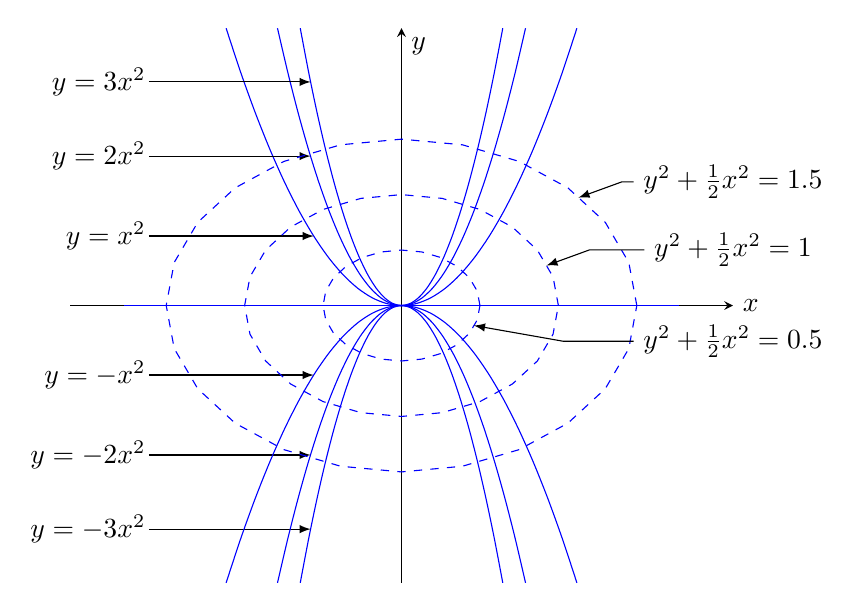
\begin{tikzpicture}
    \begin{axis}[axis equal,clip=false,
            xtick=\empty,
            ytick=\empty,
            axis lines =middle, xlabel=$x$, ylabel=$y$,
            every axis x label/.style={at=(current axis.right of origin),anchor=west}
          ]

    \pgfplotsinvokeforeach{-3,-2,...,2,3}{
     \ifnum #1 = 0
       \addplot [blue, smooth,domain=-2.5:2.5] {#1*x^2} coordinate[pos={0.2}] (n#1);
     \else
       \addplot [blue, smooth,domain={-sqrt(2.5/abs(#1))}:{sqrt(2.5/abs(#1))}] {#1*x^2} 
       coordinate[pos=0.45-0.12*abs(#1)] (n#1);
     \node[inner sep=1pt,anchor=east,] (nn#1) at ([xshift=1cm]current axis.west|-n#1) 
     {$y=\ifnum#1=1
     \else 
     \ifnum#1=-1
     -\else
     #1
     \fi\fi x^2$};
     \draw[-latex,thin] (nn#1) -- (n#1);
     \fi
    }
   \addplot [blue,domain=0:360,dashed] ({.5*sqrt(2)*cos(x)},{.5*sin(x)})
   coordinate[pos=0.95] (e0);
   \addplot [blue,domain=0:360,dashed] ({sqrt(2)*cos(x)},{sin(x)})
   coordinate[pos=0.05] (e1);
   \addplot [blue,domain=0:360,dashed] ({1.5*sqrt(2)*cos(x)},{1.5*sin(x)})
   coordinate[pos=0.1] (e2);
   \path ([yshift=-2mm]current axis.east|-e0)  node (ne0) {$y^2+\frac{1}{2}x^2=0.5$}
   ([yshift=2mm]e1-|current axis.east)  node  (ne1){$y^2+\frac{1}{2}x^2=1$}
   ([yshift=2mm]e2-|current axis.east)  node  (ne2) {$y^2+\frac{1}{2}x^2=1.5$};
 \end{axis}
   \foreach \X in {0,1,2}
   {\draw[latex-,thin] (e\X) to[connect with angle={-10+30*sign(\X)}]  (ne\X.west);}
\end{tikzpicture}

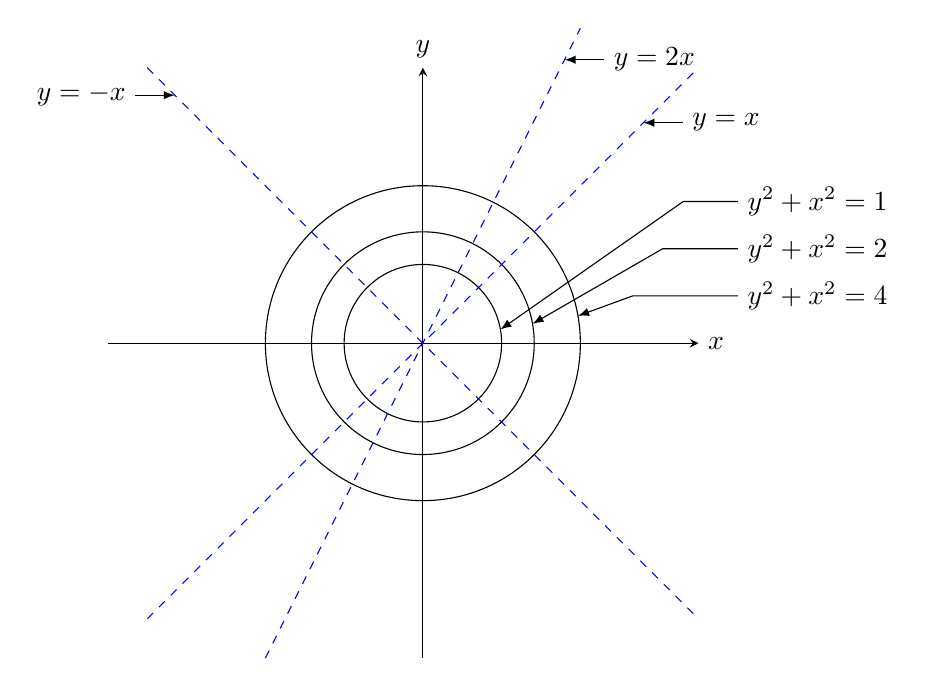
\begin{tikzpicture}
  \draw [-stealth] (-4,0) -- (3.5,0) node [right] {$x$};
  \draw [-stealth] (0,-4) -- (0,3.5) node [above] {$y$};
  \foreach \X in {1,2,4}
  {\draw (0,0) circle[radius={sqrt(\X)*1cm}] (10:{sqrt(\X)})coordinate (c\X);}
  \draw [dashed,blue] (-3.5,-3.5) -- (3.5,3.5) coordinate[pos=0.9] (x2)
   (-3.5,3.5) -- (3.5,-3.5) coordinate[pos=0.05] (x1)
   (-4/2,-4) -- (4/2,4) coordinate[pos=0.95] (x3);
  \draw[latex-,thin] (x1) -- ++ (-0.5,0) node[left]{$y=-x$};
  \draw[latex-,thin] (x2) -- ++ (0.5,0) node[right]{$y=x$};
  \draw[latex-,thin] (x3) -- ++ (0.5,0) node[right]{$y=2x$};
  \path (4,0.6) node[right] (r4) {$y^2+x^2=4$};
  \path (4,1.2) node[right] (r2){$y^2+x^2=2$};
  \path (4,1.8) node[right] (r1) {$y^2+x^2=1$};
     \foreach \X in {1,2,4}
     {\draw[latex-,thin] (c\X) to[connect with angle={40-\X*5}]  (r\X.west);}
\end{tikzpicture}

\end{document} 